\documentclass{article}

\usepackage{arxiv}

\usepackage[utf8]{inputenc} % allow utf-8 input
\usepackage[T1]{fontenc}    % use 8-bit T1 fonts
\usepackage{hyperref}       % hyperlinks
\usepackage{url}            % simple URL typesetting
\usepackage{booktabs}       % professional-quality tables
\usepackage{amsfonts}       % blackboard math symbols
\usepackage{nicefrac}       % compact symbols for 1/2, etc.
\usepackage{microtype}      % microtypography
\usepackage{lipsum}
\usepackage{graphicx}
\graphicspath{ {./images/} }

\usepackage{amsmath}  
\usepackage{amsfonts} 
\usepackage{graphicx}
\graphicspath{ {./images/} }
%\usepackage[demo]{graphicx}
\usepackage[usenames]{color}
\usepackage{mathtools}
\usepackage{algorithm}
\usepackage[noend]{algpseudocode}
\usepackage{float}
\usepackage{xcolor}
\usepackage{comment}


\DeclarePairedDelimiter{\abs}{\lvert}{\rvert}
\DeclareMathOperator{\esssupp}{ess\,supp}

\lineskip=1.5\lineskip


% MATH -----------------------------------------------------------
\newcommand{\Real}{\mathbb R}
\newcommand{\eps}{\varepsilon}
\newcommand{\diag}{\mathrm{diag}}
\newcommand{\nbr}{\mathrm{nbr}}
\newcommand{\F}{\mathcal{F}}
\newcommand{\Hil}{\mathscr{H}}
\newcommand{\LL}{\mathcal{L}}
\newcommand{\G}{\mathscr{G}}
\newcommand{\s}{\mathbb{S}}
\newcommand{\p}{\mathscr{P}}
\newcommand{\C}{\mathscr{C}}
\newcommand{\one}[1]{\mathbf{1}_{\{#1\}}}
\newcommand{\oneset}[1]{\mathbf{1}_{#1}}
\renewcommand{\P}{\mathbb{P}}
\newcommand{\Q}{\mathsf{Q}}
\newcommand{\E}{\mathbb{E}}
\newcommand{\osimplex}{\mathcal{S}^{d-1}}
\newcommand{\csimplex}{\bar{\mathcal{S}}^{d-1}}
\newcommand{\argmin}{\mathrm{argmin}}
\newcommand{\argmax}{\mathrm{argmax}}
\newcommand{\var}{\mathrm{Var}}
\newcommand{\cov}{\mathrm{Cov}}
\newcommand{\ind}{\mathrm{I}}
\newcommand{\Borel}{\mathscr{B}}
\newcommand{\M}{\mathcal{M}}
\newcommand{\Z}{\mathcal{Z}}
\renewcommand{\d}[1]{\ensuremath{\operatorname{d}\!{#1}}}
\newcommand{\D}{\mathrm{d}}

\newcommand{\ds}{\displaystyle}

\DeclareMathOperator{\trace}{tr}
\DeclareMathOperator*{\esssup}{ess~sup}
\DeclareMathOperator*{\essinf}{ess~inf}
\DeclareMathOperator*{\diam}{diam}
\DeclareMathOperator*{\ROC}{ROC}
\DeclareMathOperator*{\sinc}{sinc}
\DeclareMathOperator*{\sign}{sign}
\newcommand{\voila}{\hfill $\blacksquare$}
\newcommand{\Id}{\mathrm{Id}}
\newcommand{\K}{\mathbb{K}}
\renewcommand{\Re}{\mathrm{Re}}
\renewcommand{\vec}[1]{\mathbf{#1}}
\newcommand*\diff{\mathop{}\!\mathrm{d}}




\title{Novel methodology for the reconstruction of a partially observed biological invasion}


\author{
 Valentina Di Marco  \\
  School of Mathematical Science\\
  Monash University, Clayton Campus\\
  VIC 3800, Australia \\
  \texttt{valentina.dimarco@monash.edu} \\
  %% examples of more authors
  \And
 Jonathan Keith \\
  School of Mathematical Science\\
  Monash University, Clayton Campus\\
  VIC 3800, Australia \\
  \texttt{jonathan.keith@monash.edu} \\
  \And
 Daniel Spring  \\
  Centre of Excellence in Biosecurity Risk Analysis\\
  University of Melbourne, Parkville\\
  VIC 3052, Australia \\
  \texttt{daniel.spring@unimelb.edu.au} \\
}

\begin{document}
\maketitle

\begin{abstract}
    The spread of invasive species to new areas disrupts the equilibrium of the native ecosystem and can have adverse effects on the economy and the environment of the affected region. The real extent of the invasion is often unknown, because not all individuals are detected, and this makes planning effective eradication programs difficult. The history of the invasion is usually also only partially known, so determining the real effects of past eradication efforts can be hard. 

    Rebuilding the history of a partially observed system is useful in many contexts, but in this paper we are focusing on invasive species and in particular on one of the world's 100 worst invaders: the Red Imported Fire Ants (RIFA). 

    We first introduce a new model for the RIFA invasion based on a self-exciting spatio-temporal process and then apply a novel Sequential Importance Sampling methodology to infer the locations of unobserved nests, updating the inference each time we receive a new set of observations.
\end{abstract}


\section{Introduction}\label{section:introduction}
The Red Imported Fire Ant \textit{Solenopsis Invicta} Buren \cite{GISD} or RIFA is native to South America and has spread globally \cite{Wetterer}, negatively impacting human health, public safety, ecosystems and agriculture. Distribution currently includes the United States, Australia, New Zealand, China, Malaysia, Singapore and the West Indies \cite{Wang} \cite{GISD}. In Australia it has been introduced in seven locations over the period 2001-2016 \\ \cite{WylieMay16}, and while the National Red Imported Fire Ant Eradication Program eliminated six of these incursions, the remaining one originated in Brisbane had a ``footprint" of 4,000 $\text{km}^2$ in 2015. The eradication program successfully managed to reduce the spread of the invasion, which otherwise would have covered an area of 48,000 $\text{km}^2$ according to one estimate \cite{Wylie2020}. However, a complete eradication has not yet been achieved and the current boundary of the invasion is unknown due to a lack of a monitoring activity near the previous boundary.

Complete eradication of an invasive species is usually difficult and the success of an eradication program depends on many factors including how early the first detection of the invasion occurred. When large areas are potentially infested and surveillance with limited resources is required to determine where to apply treatment, eradication can take decades, if it succeeds at all. Some areas that might be infested are not regularly surveyed owing to the high cost of monitoring, and some individuals in surveyed locations are missed because surveillance methods are imperfect \cite{Royle}, therefore observations are “incomplete”. These two factors create uncertainty about whether eradication efforts will succeed  \cite{Keith}. Understanding and correctly modelling the true extent of an invasion is fundamental to evaluate correctly how successful an eradication program is and whether or not to continue with current eradication methods. 

Our new Sequential Importance Sampling (SIS) strategy aims to assess the current extent of an invasion, imputing missing data in the presence of incomplete observations made sequentially in time. After receiving data regarding the location of some of the nests, we simulate the locations of the unknown number of undetected colonies. When new observations are made, our simulations can be improved by taking into account these new observations. We propose a two-step iterative process in which states of the system are alternatively simulated in accordance with past observations, then corrected in light of the newly received observations. As is typical of SIS methods, we generate a population of particles, each representing a plausible sequence of system states, and we evolve each particle at each time step according to a model of system dynamics. When new observations arrive in real time we use these observations to adjust the weights assigned to particles. The crucial new element in our method is that we allow missing values imputed at earlier time steps to be corrected to improve the quality of our estimation over the entire history of the invasion.

In this paper we also propose a new model for the RIFA invasion based on a self-exciting point process. A self-exciting point processes or Hawkes process \cite{Hawkes71} is a counting process modelling a sequence of events usually over a continuous time. Each of these events will influence the short-term probability of future events occurring, in the sense that the likelihood of a new event is increased for some time after the first arrival. Hawkes processes have been used in a variety of fields, from seismic activities (\cite{Ogata88}) to neuroscience (\cite{Reynaud}, \cite{Chornoboy}), crime prediction (\cite{Mohler13}, \cite{White} \\ \cite{Reinhart2018}) and social media (\cite{Chen}). Another interesting and application is in modelling the spread of diseases, for example \cite{Browning} have recently been modelling retrospectively daily counts of deaths during the COVID-19 pandemic outbreak using a time-discrete Hawkes process.

Self-exciting models are not extensively used in the study of invasive species. An issue that arises in these kind of applications is that often data is organized into counts of observations within predefined grid cells. Spatio-temporal self-exciting point processes are useful when the locations of individuals are exactly recorded, so the spatial distribution of the invaders can be considered a point process. Balderama, Schoenber and Murray \cite{Balderama} presented an interesting first application of Hawkes processes as branching models to the study of the incidence of invasive plant and animal species. In 2017 Gupta, Farajtabar, Dilkina and Zha \cite{Gupta} published a paper where they applied Hawkes processes to invasive species management. Our paper is a third application of self-exciting point processes to invasive species. 

Other methods have been put forward for the reconstruction of the RIFA invasion in Australia. Keith and Spring \cite{Keith} proposed an agent-based model for the RIFA invasion focused on reconstructing the historical trajectory of the invasion to determine if the eradication strategy then applied was successful. Their method consisted of constructing a likelihood model in terms of some unknown parameters that included, among other things, the phylogeny, jump type, founding type and treatment success rate. They then constructed the dependencies among the known and unknown parameters and defined all conditional distributions. The posterior distribution was then sampled using a generalised Gibbs technique \cite{Keith2004} that enables transdimensional sampling. This technique is useful when the number of parameters is unknown, as in their case.
In our new approach, we are seeking to simplify and improve on the model of Keith and Spring \cite{Keith}, with the aim to reduce the running time without compromising on flexibility and completeness.

The new SIS method is an efficient way to recalculate particle weights as new observations arrive, in particular because previous estimates can be updated in light of new data, thus addressing a major limitation of the MCMC approach, which requires the entire inference process to be started from scratch each time new data becomes available.






\section{The self-exciting point process}\label{section:model}

Here we present a first application of a self-exciting point process to the modelling of insect invasion. Two key aspects of our application are that we consider the detection process in parallel with the founding event and that we include unobserved nests alongside observed nests in the detection likelihood to model the missing data.

Firstly we introduce the self-exciting spatio-temporal point process that generalises an Hawkes model \cite{Hawkes71} for one time iteration. This model involves an intensity function $\lambda(x, y, t)$, which represents the infinitesimal expected rate of events at time $t$ and location $(x, y)$, given all the events up to time $t$.

Let $\mathcal{F}$ be a $\sigma$-algebra on $\Omega = S \times [0, \infty )$, where $S$ is a bounded region of $\mathbb{R}^2$ and $[0, \infty)$ is the temporal domain. Let $N: \mathcal{F} \to \mathbb{R}$ be a counting measure, with $N(A)$ representing the number of points in $A$ for $A \in \mathcal{F}$. More precisely, suppose $N$ is a random counting measure, where a random measure is a map from a probability space $(\Omega, \mathcal{F}$, \mathbb{P}) to a measurable space $(N_{X}, \mathcal{B}(N_{X}))$ where $N_{X}$ is the space of all boundedly finite integer-valued measures (\cite{Daley}, chapter 6). The function $g(x - x', y - y', t - t')$  is the clustering density (or excitation function or triggering function), with $t'$ the time of founding of a parent nest with spatial coordinates $s' = (x', y')$. {\color{red} This function, centered at the triggering event, is the intensity function for the offspring process (or excitation process). Properly normalized, it induces a probability distribution for the location and times of the offspring events.}

We can then write the intensity function for new nests, conditional over the past history of the process $\mathcal{H}_t$, in terms of a stochastic integral:

\begin{equation}\label{eq:intensity}
    \lambda(x, y, t | \mathcal{H}_t) = \mu(x, y, t) + \int_{0}^{t} \iint_{S} g(x - x', y - y', t - t') \d N(x', y', t')
\end{equation}
were $\d N(x', y', t') = 1$ if the infinitesimal element $\d N(x', y', f')$ contains a parent and is 0 otherwise. $\lambda(x, y, t)$ may be thought of as the frequency with which events are expected to occur around a particular location $(x, y, t)$ in space–time.

Since N is a counting measure, we can write equation (\ref{eq:intensity}) as

\begin{equation*}
    \lambda(x, y, f) = \sum_{ p: f_p < f } g \Big(x - x_p, y - y_p, f - f_p \Big)
\end{equation*}
where the subscript $p$ represent the parent nest.

In our model the temporal behavior of the process is independent of the spatial behavior so we can write

\begin{equation*}
    \lambda(x, y, f | \mathcal{H}_f) = \mu(x, y, f) + \sum_{ p: f_p < f } r(f-f_p) l\Big((x - x_p), (y - y_p)\Big)
\end{equation*}
where $r$ and $l$ are known as the {\em triggering functions} for time and space respectively. From now on we will omit the explicit conditioning on the past history $\mathcal{H}_f$ for ease of notation.

New individuals from the invasive species can be introduced at any time by carriers like animals or humans. For simplicity, in the RIFA invasion we will assume that there are no exogenous introductions and we will therefore set the background term $\mu(x, y, f) $ equal to 0.

Each parent nest is able to found more than one nest, with the number of nests founded per nest per month being a parameter $\zeta$. Also, the nests have a maturation time $t_m$ of 8 months, meaning that before reaching this age they will not be able to produce new nests. therefore the temporal triggering kernel will be the function
{\color{red}
\begin{equation*}
    r (f - f_p | \zeta) =
    \begin{cases}
        0, & \mbox{if} \quad f - f_p < t_{m} \\
        \zeta, & \mbox{if} \quad f - f_p \geq t_{m}
    \end{cases}
\end{equation*}}
where $f$ is the founding time of the new nest and $f_p$ is the founding time of the parent nest.

Biological invasions spread via local movements and by long-distance jumps \cite{Suarez}. The long distance jumps are often human-assisted and create new clusters far from the founding cluster. We therefore consider two founding types: a local founding event represented by $U_i = 0$ and a long-distance jump represented by $U_i = 1$ with $i=\{1, \dots, N\}$. The vector of jump types is $U = (U_1, \dots, U_N)$, with $N$ the total number of founded nests.

The vector of jumps types has probability density function

\begin{equation*}
    p(U| \gamma ) = {N \choose \nu}(\gamma)^{2\nu}(1 - \gamma)^{2(N - \nu)}
\end{equation*}
where $\gamma$ is the probability of a long jump (VVV note that I don't have this number. For the simulation I am using 1\%. HHH Do you infer this number? Or assume it is known? {\color{red} VVV infer this number from first year of data}) and $\nu$ is the number of long-distance jumps.

For newly founded nests we model the distribution of radial distance from the parent nest as an exponential distribution for the local founding event and a L\'evy distribution for the long-distance jumps. The distribution over the angular direction will be uniform as it is equally possible to found a nest in every direction from the parent nest. Therefore the probability distributions for the short jumps ($l_0$) and for the long jumps ($l_1$) are

\begin{equation*}
    l_0\Big((x - x_p), (y - y_p) | U, \sigma \Big)= J \bigg(\frac{1}{2 \pi} \sigma e^{- \sigma r}\bigg)
\end{equation*}

\begin{equation*}
    l_1\Big((x - x_p), (y - y_p) | U, c \Big)= J \bigg(\frac{1}{2 \pi} \sqrt{\frac{c}{2 \pi}} \frac{e^{- \frac{c}{ 2 r}}}{r^{3/2}}\bigg)
\end{equation*}
where $J$ is the Jacobian of the trasfomation from polar coordinated to cartesian coordinates and $r$ is the radial distance between a parents nest and a newly founded nest.

We also make the assumption that nests are killed as soon as they are detected. {\color{red} This is not usually the case as normally only a portion of the observed nests are successfully eliminated, but here we make this assumption for simplicity.} so we introduce an indicator function $I(t_d - t)$ such that

\begin{equation*}
    I (t_d - t) =
    \begin{cases}
        1, & \mbox{if} \quad t_d -  t> 0 \\
        0, & \mbox{otherwise}
    \end{cases}
\end{equation*}
where $t_d$ represents the time of detection. So the conditional intensity function is

{\color{red}
\begin{equation*}
    \lambda(x, y, t) = \sum_{p:f_p < t} r(t - f_p | \zeta) I((t_d)_p - t) p(U | \gamma) l_0(x, y | U, \sigma) l_1(x, y | U, c)
\end{equation*}}
where we must have $f_p\leq (t_d)_p$. (HHH $\lambda$ now has an additional argument $t$ that it didn't have before. Should it be conditioned on $t$? Also, each nest has a different $t_d$, so should it have a subscript $p$?)

As demonstrated by Hawkes and Oakes \cite{Hawkes74}, any stationary self-exciting point process with finite intensity may be interpreted as a Poisson cluster process with the number of offspring for each event drawn from a Poisson distribution with mean 

\begin{equation} \label{eq:NumOffsp}
    {\color{red} m = \int_0^{T} \iint_S g(x, y, t)\d x \d y, \d t = \zeta \kappa T}
\end{equation}
{\color{red} where $\kappa$ is the number of parents nests that were unobserved and mature by time $T$. VVV I wrote the integral wrong here, this should be right now}

{\color{red} ..... Let us assume that each parent nest alive from the previous time produces zero or more nests independently of one another, and the number of newly founded nests form an inhomogeneous Poisson process. The rate at which the parent $p$ will produce offspring at time $t > f_p$ is $g(t - f_p)$. The direct offspring of this individual comprise the first generation and their offspring the second generation and so on. The descendants of this parent nest $p$ are the memebers of the union of all these generations). If we define with $Z_p$ the random number of offspring in the  ..... }
(HHH The preceding sentence needs to be expanded to a paragraph or more. Explain what a Poisson cluster process is, and how it differs from a Poisson point process. Explain what the events are, in particular making clear what you mean by ``the number of offspring for each event''. You might want to reuse parts of your literature review to explain these processes in detail.)
The joint probability or likelihood at time $T$ is that of an inhomogeneous Poisson process for the founding process with intensity $\lambda(x, y, t)$ (See Reinhart \cite{Reinhart} for a derivation of the likelihood for self-exciting spatio-temporal point processes HHH Consider adding an equation for the likelihood derived there).

We will now consider the detection processes in parallel with the founding processes, in a similar way to Jewell's model for infectious diseases \cite{Jewell}. This facilitates including unobserved nests alongside observed nests in the detection likelihood to fully model the missing data. We will treat the time from {\color{red}founding to detection} $(t_i - f_i)$ of an offspring nest $i$ as a random variable exponentially distributed with parameter $\varphi$

\begin{equation*}
    h(t_{i} - f_{i} | \varphi) = \varphi \exp (- \varphi(t_{i} - f_{i})).
\end{equation*}
The Likelihood of a set of $n$ {\color{red} observed nests, whose locations are} $(s_{1}, ... , s_{n})$ with $s_i = (x_i, y_i)$ {\color{red}and whose founding times and detection times are respectively} $(f_{1}, ... , f_{n})$ and $(t_{1},  ... , t_{n})$ will then be:

\begin{equation} \label{eq:like}
    \begin{aligned}
        L(s_{1}, ..., s_{n}, f_{1}, ..., f_{n}, t_{1}, ..., t_{n} ; \Theta) = & \Bigg[ \prod_{i = 1}^{n} \lambda(s_{i}, t_{i}, f_{i}) \Bigg] \exp \Bigg(- \int_{0}^{T} \int_{0}^{T} \int_{S} \lambda(s, t, f) \d s \d t \d f \Bigg) \\ 
        & \prod_{\{ i : t_{i} < T \} } h(t_{i} - f_{i}) \prod_{ \{ i : t_{i} = \infty \} } \int_{T}^{\infty} h(t - f_{i}) \d t
    \end{aligned}
\end{equation}
where $t_{i} = \infty$ if nest $i$ has not been detected at time $T$ and $n$ is the number of nests founded. The quantity $h(t_{i} - f_{i})$ is the contribution {\color{red} to the likelihood} of the observed nests, while $\int_{T}^{\infty} h(t - f_{i}) \d t$ is the contribution {\color{red} to the likelihood} of the unobserved nests. The vector of parameters is $\Theta = ( \sigma, c, \gamma, \zeta, \varphi)$.

The term 

\begin{equation*}
    \exp \bigg(- \int_{0}^{T} \int_{S} \lambda(s, t)\d s \d t \bigg)
\end{equation*}
in the likelihood will evaluate to 

\begin{equation*}
    \exp \bigg(- \zeta \sum_{i=1}^{n} (min\{ T, t_i \} - f_i) \bigg)
\end{equation*}
as the spatial part evaluates to 1 and the temporal part is constant over the lifetime of each nest. Substituting the function $h$ and evaluating the last integral in (\ref{eq:like}) we get

\begin{equation*}
    \begin{aligned}
        L = & \Bigg[ \prod_{i = 1}^{n} \lambda(s_{i}, t_{i}, f_{i}) \Bigg] \exp \bigg(- \zeta \sum_{i=1}^{n} (min\{ T, t_i \} - f_i) \bigg) \\ 
        & \prod_{\{ i : t_{i} < T \} } \varphi \exp (- \varphi (t_{i} - f_{i})) \prod_{ \{ i : t_{i} = \infty \} } \exp \bigg( - \varphi(T - f_{i}) \bigg).
    \end{aligned}
\end{equation*}
It is also useful to define the log-likelihood

\begin{equation*}
    \begin{aligned}
        L_{log} = & \Bigg[ \sum_{i = 1}^{n} \log \lambda(s_{i},f_{i}, t_{i}) \Bigg] - \bigg(\zeta \sum_{i=1}^{n} (min\{ T, t_i \} - f_i) \bigg)  + \sum_{\{ i : t_{i} < T \} }  \bigg[\log (\varphi) -\varphi(t_{i} - f_{i}) \bigg] \\
        - & \sum_{ \{ i : t_{i} = \infty \} } \bigg[\varphi(T - f_{i}) \bigg].
    \end{aligned}
\end{equation*}
Notice that natural deaths are not considered in our model, so nests are treated as if immortal unless detected and removed.







\section{Model simulation} \label{section:simulationModel}

{\color{red} Let us define the intervals $\tau_j = (T_{j-1}, T_j]$ where $T_j$ is the time at which we receive a new set of observations, so the time interval $[T_0, T_i]$ from the beginning of the invasion $T_0=0$ to the time of the last detection $T_i$ will be partitioned into sub-intervals $\tau_j$ with $j = 1, \dots, i$. Each nest ever created up to time $T_j$ will be represented by $a^{T_j}_k = (t_k^{T_j}, f_k^{T_j}, x_k^{T_j}, y_k^{T_j})$ where $f_k$ is the time of founding, $t_k$ is the time of observation corresponding to the time of death, and $x_k$ and $y_k$ are the spatial coordinates.}

To simulate the process in each of these time intervals $\tau_j$ we will view the model as a branching Poisson process \cite{Lewis}, which is a natural choice for invasive species. This immigration-birth representation {\color{red}in which each immigrants arrive at times given by a Poisson process then starts a new generation which will generate new offspring and so on,} gives rise to a simpler simulation procedure than the thinning algorithm introduced by Ogata \cite{Ogata81}. A procedure of this kind was introduced by Zhuang \cite{Zhuang} for self-exciting spatio-temporal point processes in the context of earthquake models. The simulation proceeds as follows:

\begin{enumerate}
    \item Consider the catalogue of events $G^{T_{j-1}}$ (HHH Define this mathematical object more precisely.) which contains the nests that have not been observed and killed at or before time $T_{j-1}$. Take all the unobserved nests that will be mature (older than 8 months) by time $T_j$ and put them in the catalogue $G_l^{T_j}$.
    \item Set $l = 0$.
    \item From $G_l^{T_j}$ select which nests are mature and put in catalogue $M_l^{T_j}$ (HHH Define. Do you remove it from $G_l^{T_j}$ when you add it to $M_l^{T_j}$?).
    \item For each nest in $M_l^{T_j}$ simulate (HHH Consider using the word `draw' instead of `simulate', where that's an appropriate substitution) the number of offspring $\eta^{T_j}$ produced in the time interval $\tau_j$ from a Poisson distribution with parameter $ m^{T_j} = \zeta (T_j-t_m)$ where $m^{T_j}$ was defined in equation (\ref{eq:NumOffsp}).
    \item Simulate for each of the offspring the time of founding from a uniform distribution that is $1/(T_j-t_m)$ if $t_m \leq f - f' \leq T_j$ and $0$ otherwise.
    \item Simulate the number of long-distance jumps $\mu^{T_j}$ from a binomial distribution with probability $\gamma$ and total number of offspring $\eta^{T_j}$.
    \item Simulate the location of these offspring. This is done by simulating the angular direction and the radial direction separately, then calculating the coordinates $x$ and $y$. The angular direction will be simulated from a uniform distribution in the interval $(0, 2\pi]$. The radial direction for the long jumps will be simulated from a L\'evy distribution with parameter $c$ (VVV the bigger this parameter the higher the jumps simulated). The radial direction for the cluster events will be simulated from a decaying exponential distribution with parameter $\rho$. (HHH I don't think `radial direction' is a clear descriptor in this point. Perhaps you mean `founding distance'?)
    \item Simulate for each offspring the time from establishment to notification from an exponential distribution with parameter $\varphi$.
    \item Delete (HHH from what?) all parent nests that have been observed in the time interval $\tau_j$.
    \item Store each newly generated and not yet observed nest's location, time of founding and time of observation in $O_l^{T_j}$. Let $G_{l}^{T_j} = \bigcup_{k=1}^{\eta^{T_j}} (O_l^{T_j})_k$. (HHH Define.)
    \item If $G_l^{T_j}$ is not empty, set $l = l+1$ and return to step 3. Otherwise return $\bigcup_{h=0}^l G^{T_j}_h$ as the final set of simulated events for the time interval $\tau_j$.
\end{enumerate}

(HHH A brief, small-scale example would help here.)






\section{Sequential Importance Sampling with corrections applied to the self-exciting point process} \label{sec:SISMethod}

In this section we apply a new Sequential Importance Sampling methodology to the model above in order to estimate position and time of founding of all observed and unobserved nests. As we have discussed in the introduction, during the eradication program locations of nests are continuously acquired either through passive or active surveillance (HHH define these somewhere) activities, while new nests are also continuously created (HHH founded?). We consider the locations and time of observation as exact measurements, however, only a limited number of colonies (HHH Is a colony different from a nest?) will be detected at each observation time while an unknown number of them will remain undetected. If an area is surveyed and deemed free of invaders, this can be because there are no invaders to be detected or because we fail to make an observation. This can happen for example when nests are young and not easy to spot. At each step we will simulate plausible locations and founding times for all the undetected nests created in the past and for all the newly created nests. When receiving new data these simulations will need correction in order to remain a plausible configuration of nests in light of the available data. We will therefore correct the simulation then adjust the weights in order to correctly represent the posterior distribution. (HHH Need to explain how particles represent a distribution.)

\subsection{Bayesian inference in a partially observed state space} \label{subsec:POS}

Consider the system of nests evolving continuously in time. The coordinates of this system are comprised of the location, time of founding and time of detection for all nests (HHH So you don't include parent of each nest? That's good, I'm just checking. What about founding type for each nest: do you include those as system coordinates? ). The states of this system at times $T_j$ are represented by random elements $\vec{a}^{T_j} = (a^{T_j}_1, \dots, a^{T_j}_{N^{T_j}}) \in \mathbb{R}^{4\times N^{T_j}}$ where $N^{T_j}$ is itself a random variable: the unknown number of nests alive at time $T_j$. Here the vectors $a^{T_j}_k = (t_k^{T_j}, f_k^{T_j}, x_k^{T_j}, y_k^{T_j})$ with $k = 1, \dots , N^{T_j}$ represent the nests indexed by $k$ and containing 4 elements: the time of founding $f_k$, the time of observation $t_k$ corresponding to the time of death, and the coordinates $x_k$ and $y_k$ (HHH This seems to repeat information: reword paragraph to avoid repetition).
The trajectory of the system from $T_0$ to $T_i$ is represented by the random element $\vec{A}^{T_i} = (\vec{a}^1, \dots, \vec{a}^{T_i})$.

We also define an \textit{observation} $\vec{z}^{T_i} \in \mathbb{R}^{i \times M^{T_i} \times 3}$ (HHH I don't understand why $i$ is a factor in the exponent there.) where $M^{T_i}$ is the total number of nests detected up to time $T_i$. Note $M^{T_i}$ is also a random variable, but its value is observed at time $T_i$. The elements of $\vec{z}^{T_i}$ are vectors $z^{T_j}_l = (t^{T_j}_l, x^{T_j}_l, y^{T_j}_l)$ containing the time of observation and coordinates of the observed nest indexed by $l$ with $l = 1, \dots, M^{T_j}$. It will also be useful to define $\vec{Z}^{T_i} = (\vec{z}^1, \dots, \vec{z}^{T_i})$. Since our observations are exact, $\vec{Z}^{T_i}$ determines the values of location and time of observation for $M^{T_i}$ nests, thus leaving $N^{T_i}-M^{T_i}$ elements of $\vec{A}^{T_i}$ completely undetermined. Moreover, the time of founding is not observed for any of the nests. Thus even the co-ordinates $a^{T_j}_k$ of a detected nest are only partially determined by an observation. We define a function $\sigma_{T_i}: \mathbb{R}^{i\times N^{T_j}\times 3} \rightarrow \mathbb{R}^{i\times M^{T_j}\times 4}$ such that $\vec{Z}^{T_i} = \sigma_{T_i}(\vec{A}^{T_i})$. (HHH I don't understand why there is an $i$ in each of the exponents, and the arrow seems to be going the wrong way. Also, the function $\sigma_{T_i}$ needs an additional argument to determine which nests are observed.)

Using a Bayesian approach, we can quantify our state of knowledge of the system at time $T_i$ using a posterior distribution, conditional on the model of the system and the data received.

At time $T_1$ our knowledge of the system is represented by a prior distribution with density $q(\vec{A}^{T_1})$ on $\Omega_{T_1} = \mathbb{R}^{N^{T_1}}$ (HHH Why no '4'?) and the posterior distribution after observing $\vec{Z}^{T_1}$ has density on $\Omega'_{T_1} = \sigma_{T_1}^{-1}(\vec{Z}^{T_1})$ given by:

\begin{equation*}
    p(\vec{A}^{T_1} | \vec{Z}^{T_1}) = \frac{q(\vec{A}^{T_1})}{r(\vec{z}^{T_1})}
\end{equation*}
where
\begin{equation*}
    r(\vec{z}^{T_1}) = \int_{\Omega'_{T_1}} q(\vec{A}^{T_1}) 
\end{equation*}
and the integral is over the elements of $\vec{A}^{T_1}$ that are not determined by $\vec{Z}^{T_1}$.

(HHH The prior and posterior distributions will need to include a random variable indicating which nests are observed.)

(NOTE: I need to define the metric here. I think it would be good to explain this exactly as Jon has done in his original notes on the method with the disintegration theorem. I guess this will perhaps depend on which journal we are going to submit the paper to). (HHH Do you mean `measure', rather than `metric'?)
Our knowledge of the trajectory of the system at time $T_j$ with $i \geq 2$, before we acquire the next set of observations $\vec{z}^{T_i}$, is represented by a prior distribution with density $q(\vec{A}^{T_i} | \vec{Z}^{T_{i-1}})$ on the subspace $\Omega_{T_i} = \sigma_{T_i}^{-1} (\vec{Z}^{T_{i-1}}) \times \mathbb{R}^{4 \times N^{T_i}}$. After observing $\vec{z}^{T_i}$, $N^{T_i}$ elements of $\vec{A}^{T_i}$ with non zero prior density will be revealed, and the posterior density must restrict $\vec{A}^{T_i}$ to $\Omega_{T_i}' = \sigma_{T_i}^{-1}(\vec{Z}^{T_i})$. The posterior density over $\Omega_{T_i}'$ will then be

\begin{equation*}
    p(\vec{A}^{T_i} | \vec{Z}^{T_i}) = \frac{q(\vec{A}^{T_i} | \vec{Z}^{T_{i-1}})}{r(\vec{z}^{T_i} | \vec{Z}^{T_{i-1}})}
\end{equation*}
were

\begin{equation*}
    r(\vec{z}^{T_i} | \vec{Z}^{T_{i-1}}) = \int_{\Omega'_{T_i}} q(\vec{A}^{T_i} | \vec{Z}^{T_{i-1}}).
\end{equation*}
Let $L(\vec{a}^{T_i} | \vec{a}^{T_{i-1}})$ be the density distribution characterising the system which is the joint probability distribution we have defined in equation (\ref{eq:like}) chapter  \ref{section:model}. The system we are considering, which includes location, time of founding and time of observation of the nests, is Markovian, that is, each $\vec{a}^{T_i}$ is conditionally independent of $\vec{A}^{T_{i-2}} = (\vec{a}^{T_1}, \ldots,\vec{a}^{T_{i-2}})$, given $\vec{a}^{T_{i-1}}$.

It follows that at time $T_1$ the joint prior distribution for $\vec{A}^{T_1}$ will be

\begin{equation*}
    q(\vec{A}^{T_1}) = L(\vec{a}^{T_1}),
\end{equation*}
and for $T_i$ with $i \geq 2$

\begin{equation*}
    q(\vec{A}^{T_i} | \vec{Z}^{T_{i-1}}) = L(\vec{a}^{T_i} | \vec{a}^{T_{i-1}}) p(\vec{A}^{T_{i-1}} | \vec{Z}^{T_{i-1}}) = \frac{L(\vec{a}^{T_1})}{r(\vec{z}^{T_1})} \prod_{j=2}^{i-1} \frac{L(\vec{a}^{T_j} | \vec{a}^{T_{j-1}})}{r(\vec{z}^{T_j} | \vec{Z}^{T_{j-1}})} \times L(\vec{a}^{T_i} | \vec{a}^{T_{i-1}})
\end{equation*}
on the space $\Omega_{T_i}$, so the joint posterior distribution will be

\begin{equation*}
    p(\vec{A}^{T_i} | \vec{Z}^{T_i}) = \frac{L(\vec{a}^{T_1})}{r(\vec{z}^{T_1})} \prod_{j=2}^{i} \frac{L(\vec{a}^{T_j} | \vec{a}^{T_{j-1}})}{r(\vec{z}^{T_j} | \vec{Z}^{T_{j-1}})}
\end{equation*}
on $\Omega'_{T_i}$.

We will now want to approximate the distribution $p(\vec{A}^{T_i} | \vec{Z}^{T_i})$ by iterative sampling and obtain Monte Carlo Estimates of expectations of the form:

\begin{equation*}
    E_p[\alpha(\vec{A}^{T_i}) | \vec{Z}^{T_i}] = \int_{\Omega'_{T_i}} \alpha(\vec{A}^{T_i}) p(\vec{A}^{T_i} | \vec{Z}^{T_i})
\end{equation*}
for functions $\alpha : \Omega'_{T_i} \rightarrow \mathbb{R}$.
We take a Sequential Importance Sampling approach, at each iteration using a collection of weighted particles to approximate the posterior $p(\vec{A}^{T_{i-1}} | \vec{Z}^{T_{i-1}})$, in the sense that these particles can be used to construct weighted Monte Carlo estimates for integrals of the above form. We evolve these under the model to create a new set of weighted particles representing the prior for iteration $T_i$, namely $q(\vec{A}^{T_i} | \vec{Z}^{T_{i-1}})$. We then correct these particles to be consistent with the new observations $\vec{Z}^{T_i}$, and adjust the weights to ensure the resulting weighted particles provide unbiased importance sampling estimates of an expectation $E_p[\alpha(\vec{A}^{T_i}) | \vec{Z}^{T_i}]$.

Consider a particle $\vec{A}_k^{T_{i-1}}$ constructed at time $T_i$, for $k = 1, \dots, n$, where $n$ is a fixed number of particles. We generate $\vec{a}^{T_{i}}_k$ for this particle by sampling from $L(\vec{a}^{T_i} | \vec{a}_k^{T_{i-1}})$. However, the new set of observations $\vec{z}^{T_i}$ are going to be inconsistent with the particles just simulated as location and time of observation of the simulated particles will most likely not correspond to the newly observed one. Also the number of nests simulated to be observed at or before $T_i$ and not yet killed might differ from the observed one. We will use the correction strategy highlighted in the following section to generate a new corrected particle $(\vec{A}')^{T_i}_k$ and improve our estimates. Note that in the following chapter we will repress the particle subscript $k$.



\subsection{The Corrections} \label{subsec:corrections}

One possible way to correct the particle $(\vec{A}^{T_{i-1}})$ would be to amend each simulated nest's position starting from the nest closer to an observed one and continuing with the next nest closer to another observed one and so on until we we have corrected all particles with all the available observations. This way we will have only one possible substitution and our corrections will be deterministic. This method, although simple, would be undefined in the remote scenario where two observations are exactly equidistant to a simulated nest. It would also discard more probable scenarios in favor of less probable one. For example, when a simulated nest is almost equidistant to two observed nests but a second simulated nest is closer to one of those observed nest, as shown in Figure \ref{fig:1}, the method would chose the less likely substitutions. (NOTE: this part is here to explain my thought process but might not be included in a paper)

\begin{figure*}
\centering
 \subfloat[A]{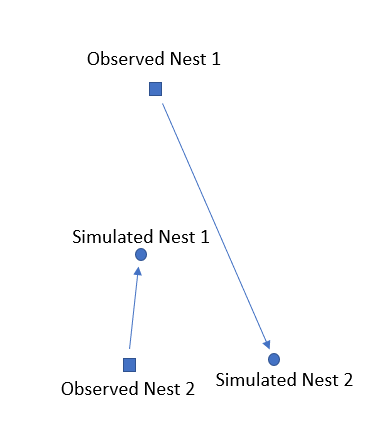
\includegraphics[width=0.3\linewidth]{subs1.PNG}}
 \subfloat[B]{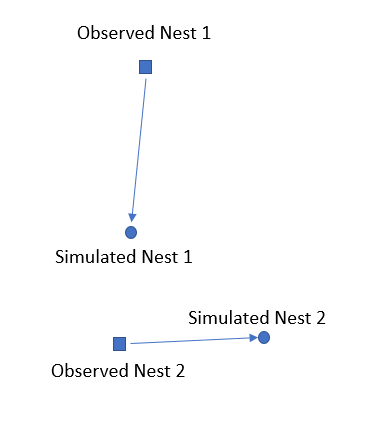
\includegraphics[width=0.3\linewidth]{subs2.PNG}}
\caption{[A] shows the shortest distance substitution in the deterministic scenario. [B] shows the more likely substitution that would be discarded in the deterministic scenario.}
\label{fig:1}
\end{figure*}

A better strategy would be the following. Assume that each particle that has been simulated up to time $T_i$ can be corrected in a finite number of ways when we receive a new set of observations $\vec{z}^{T_i}$. We also make the assumption that a nests can be only corrected once and if corrected at time $T_j$ it will not be corrected again in future times. These corrections are made with probability $H_{z^{T_i}}((\vec{A}^{T_i})' | \vec{A}^{T_i})_{\zeta}$, where $(\vec{A}^{T_i})'$ is the vector of the corrected nests at time $T_i$.

The probability $H_{z^{\tau_i}}((\vec{A}^{T_i})' | \vec{A}^{T_i})_{\zeta}$ of the new configuration of nests $\zeta$ will depend on the distances between the simulated nests and the observed nests in the following way. Let us consider a simulated nest $a_j$ and an observation $z_h$. Then $a_j$ can be corrected by $z_h$ with probability $p_{a_j z_h} = p(a_j \leftrightarrow z_h) = e^{-d_{a_j z_h}}$ where $d_{a_j z_h}$ is the Euclidean distance between $a_j$ and $z_h$. Notice that when the distance is $d_{s_j z_h} = 0$ the probability $p_{s_j z_h}$ is 1 and the observation coincide with the simulated nest. 

The probability distribution of the configurations of nests will therefore be
\begin{equation*}
    H_{z^{T_i}}((\vec{A}^{T_i})' | \vec{A}^{T_i})_{\zeta} \propto \Bigg( \prod_{h = 1}^{o^{T_i}} (p_{a_j z_h}) \Bigg)_{\zeta}
\end{equation*}
with $o^{T_i}$ the number of observed nests, and after normalization 

\begin{equation*}
    H_{z^{T_i}}((\vec{A}^{T_i})' | \vec{A}^{T_i})_{\zeta} = \Bigg(\prod_{h = 1}^{o^{T_i}} (p_{a_j z_h}) \Bigg)_{\zeta} / \sum \Bigg(\prod_{h = 1}^{o^{T_i}} (p_{a_j z_h}) \Bigg)_{\zeta}
\end{equation*} 
where the sum is over all the possible configurations. Each set of simulated particles that has not been corrected can be corrected in only a finite number of ways to produce an element of the non-empty finite set $O_{\vec{z}^{T_i}} (\vec{A}^{T_i})$ that contains all the allowed corrections. The correction is made selecting an element $(\vec{A}^{T_i})'$ from the set $O_{\vec{z}^{T_i}} (\vec{A}^T)$ with probability $H_{z^{T_i}}((\vec{A}^{T_i})' | \vec{A}^{T_i})_{\zeta}$. Configurations of nests where the distances between observed and simulated nests are small will be more probable than the one where those distances are big.

At time $T_i$, let us call $s^{T_i}$ the number of simulated nests that we want to correct. Again, $o^{T_i}$ the number of observed nests. The way we make the substitution is valid regardless of the values of $s^{T_i}$ and $o^{T_i}$ and the number of possible configurations is that obtained in ordered sampling without replacement. If we observe more nests than what we can correct the invasion can be considered eradicated. if we generate more simulated nests than observed one, we will correct only the number of nests that we observe and leave the remaining nests to be corrected at a later stage.
It follows that the number of possible configurations will be $\frac{s!}{(s-o)!}$ if $s > o$, $o!$ if $s = o$, and $\frac{o!}{(o-s)!}$ if $o < s$ (here for ease of notation we have removed the index ${T_i}$).

Each time a nest is corrected its new location will correspond to the location of one of the observed nest and the time of observation will be corrected too with the observed one.

(NOTE: This might be an expensive step if we have a large number of nests. Should we consider a threshold (for example a maximum distance) over which the substitution cannot happen?)



\subsection{The calculation of the Weights} \label{subsec:weight}

We want to simulate via a two-step process in which we generate a sample and then correct in light of data at each iteration of the Sequential Importance Sampling mechanism. To do so, we propose to use an auxiliary variable which will be the yet to be corrected sample $\vec{A}^{T_i}$, and that is an element of the probability space ($\Omega_{T_i}, \mathcal{F}, \mathbb{Q})$ where $\mathbb{Q}$ is the prior probability measure having density $q(\cdot)$. We will relate the augmented space $\Omega^*_{T_i} = \Omega_{T_i} \times \Omega'_{T_i}$ containing elements of the form $(\vec{A}^{T_i}, (\vec{A}')^{T_i})$ to the corrected state space $\Omega'_{T_i}$ containing elements of the form  $(\vec{A}')^{T_i}$ with a projection map $\pi$. 

More formally, the augmented space is defined as $\Omega^*_{T_i} = \{ (\vec{A}^{T_i}, (\vec{A}')^{T_i}) : \vec{A}^{T_i} \in \Omega_{T_i} \, , \, (\vec{A}')^{T_i} \in O_{\vec{z}^{T_i}} (\vec{A}^{T_i}) \}$. Measurable sets in $\Omega^*_{T_i}$ are of the form $\{ (\vec{A}^{T_i}, (\vec{A}')^{T_i}) : \vec{A}^{T_i} \in B \, , \, (\vec{A}')^{T_i} \in C \}$ with $B \in \mathcal{F}$ and $C \in O_{\vec{z}^{T_i}} (\vec{A}^{T_i})$ for each $(\vec{A}')^{T_i} \in B$. We denote the $\sigma$-algebra for the augmented space by $\mathcal{F}_z$ and define a reference measure on $\Omega^*_{T_i}$ for all $D \in \mathcal{F}_z$ by $\lambda_z(D) = \int_{\Omega^{T_i}} \sum_{(\vec{A}')^{T_i} \in \mathcal{F}_z(\vec{A}^T_i)} I_D((\vec{A}^{T_i}), (\vec{A}')^{T_i}) \D \lambda(\vec{A}^{T_i})$, where $I_D$ is an indicator function for $D$. The projection from the augmented space into the corrected space $\pi : \Omega^*_{T_i} \rightarrow \sigma^{-1}_{T_i}(\vec{Z}^{T_{i-1}})$ is given by $\pi((\vec{A}^{T_i}), (\vec{A}')^{T_i})) = \vec{A}^{T_i}$. 

We therefore define a probability measure $\mathbb{P}^*$ having density $p^*$ on $\Omega^*_{T_i}$ such that the marginal density of $\mathbb{P}^*$ on $\Omega'_{T_i}$ is $\mathbb{P}$, that is $\mathbb{P} = \mathbb{P}^* \circ \pi^{-1}$, where $\mathbb{P}$ is the measure with density $p$ on $\Omega'_{T_i}$.

By the disintegration theorem there exists a family of measures $\{ \nu_{(\vec{A}')^{T_i}}\}_{(\vec{A}')^{T_i} \in \Omega'_{T_i}}$ on $\Omega^*_{T_i}$ such that for every measurable Borel function $ \xi : \Omega^*_{T_i} \rightarrow [0, \infty]$

\begin{equation*}
    \int_{\Omega^*_{T_i}} \xi((\vec{A}')^{T_i}, \vec{A}^{T_i}) \D \mathbb{P}^* = \int_{\Omega'_{T_i}} \Bigg( \int_{\pi^{-1}((\vec{A}')^{T_i})} \xi((\vec{A}')^{T_i}, \vec{A}^{T_i}) \D \nu_{(\vec{A}')^{T_i}}  \Bigg) \D \mathbb{P}((\vec{A}')^{T_i}).
\end{equation*}
It follows that for any event $B$,

\begin{align*}
    \mathbb{P}(B) = \mathbb{P}^*(\pi^{-1}(B)) &= \int_{\Omega^*_{T_i}} I_B (\pi((\vec{A}')^{T_i}, \vec{A}^{T_i})) p^* ((\vec{A}')^{T_i}, \vec{A}^{T_i} | \vec{Z}^{T_i}) \D \mathbb{P}^* \\ 
    &= \int_{\Omega'_{T_i}} I_B ((\vec{A}')^{T_i}) \Bigg[ \int_{\pi^{-1}((\vec{A}')^{T_i})} p^* ((\vec{A}')^{T_i}, \vec{A}^{T_i} | \vec{Z}^{T_i}) \D \nu_{(\vec{A}')^{T_i}} (\vec{A}^{T_i}) \Bigg] \D \mathbb{P} (\vec{A}')^{T_i}.
\end{align*}
and hence

\begin{equation*}
    p((\vec{A}')^{T_i} | \vec{Z}^{T_i}) = \int_{\pi^{-1}((\vec{A}')^{T_i})} p^*((\vec{A}')^{T_i}, \vec{\vec{A}}^{T_i} | \vec{Z}^{T_i})\D \nu_{(\vec{A')}^{T_i}} (\vec{A}^{T_i}).
\end{equation*}
Moreover,

\begin{align*}
    E_{p}[l(\vec{(A')}^{T_i})]  &= \int_{\Omega'_{T_i}} l(\vec{(A')}^{T_i})\; p(\vec{(A')}^{T_i} | \vec{Z}^{T_i}) \D \mathbb{P}(\vec{(A')}^{T_i}) \\
    &= \int_{\Omega'_{T_i}} l(\vec{(A')}^{T_i})\Bigg[\int_{\pi^{-1}((\vec{A}')^{T_i})} p^*(\vec{(A')}^{T_i}, \vec{A}^{T_i} | \vec{Z}^{T_i}) \D \nu_{(\vec{A}')^{T_i}}(\vec{A}')^{T_i} \Bigg] \D \mathbb{P}{(\vec{A}')}^{T_i} \\ 
    &= \int_{\Omega^*_{T_i}} l(\pi(\vec{(A')}^{T_i}, \vec{A}^{T_i}))\; p^*(\vec{(A')}^{T_i}, \vec{A}^{T_i} | \vec{Z}^{T_i}) \D \mathbb{P}^*((\vec{A}')^{T_i}, \vec{A}^{T_i}) \\ 
    &= E_{p^*}[l(\pi (\vec{(A')}^{T_i}, \vec{A}^{T_i}))].
\end{align*}
Similarly, we define a density $\mathbb{Q}^*$ on $\Omega^*_{T_i}$ having probability function $q^*$ such that the marginal density of $\mathbb{Q}^*$ on $\Omega_{T_i}$ is $\mathbb{Q}$. We then use a sequential importance sampling approach to re-weight a sample of particle used for Monte Carlo estimation with respect to $q^*$, so that they can be used for Monte Carlo estimation with respect to $p^*$.

With the corrections introduced in chapter \ref{subsec:corrections} and reintroducing the particle subscript $k$ the joint density at $((\vec{A}_k')^{T_i}, \vec{A}_k^{T_i})$ sampled from the prior will be

\begin{equation*}
    q^*(\vec{(A')}^{T_i}_k, \vec{A}^{T_i}_k | \vec{Z}^{T_{i-1}}) = q(\vec{A}^{T_i}_k | \vec{Z}^{T_{i-1}}) H_{z^{T_i}} (\vec{(A')}^{T_i}_k | \vec{A}^{{T_i}}_k).
\end{equation*}
and the density $p^*(\vec{(A')}^{T_i}_k, \vec{A}^{T_i}_k | \vec{Z}^{T_i})$ will be

\begin{equation*}
    p^*(\vec{(A')}^{T_i}_k, \vec{A}^{T_i}_k | \vec{Z}^{T}) = p(\vec{(A')}^{T_i}_k | \vec{Z}^{T_i}) u(\vec{(A)}^{T_i}) H_{(z')^{T_i}} (\vec{A}^{T_i}_k | \vec{(A')}^{{T_i}}_k)
\end{equation*}
where we choose $u$ to be the uniform density on $\Omega'_{T_i}$ and where $H_{(z')^{T_i}} (\vec{A}^{T_i}_k | \vec{(A')}^{{T_i}}_k)$ represents a correction we would have made had we initially generated a sample $H_{(z')^{T_i}} (\vec{A}^{T_i}_k | \vec{(A')}^{{T_i}}_k)$.

(NOTE: The prof that p* is a proper density, that p* has marginal density p and the validity of the essential supports will be put in the appendix).

Applying importance sampling on the probability space $\Omega^*_{T_i}$ we have

\begin{align*}
    E_{p^*}[l(\pi (\vec{(A')}^{T_i}, \vec{A}^{T_i})] = \int_{\Omega^*_{T_i}} l(\pi((\vec{A}')^{T_i}, \vec{A}^{t})) \frac{p^*(\vec{(A')}^{T_i}, \vec{A}^{T_i}|\vec{Z}^{T_i})} {q^*(\vec{(A')}^{T_i}, \vec{A}^{T_i} | \vec{Z}^{T_{i-1}})}  \\
    q^*(\vec{(A')}^{T_i}, \vec{A}^{T_i} | \vec{Z}^{T_{i-1}}) \; \D \mathbb{P}^*((\vec{A}')^{T_i}, \vec{A}^{T_i}) \approx \sum_{i=1}^n  w^{T_i}_i l(\pi (\vec{(A')}^{T_i}_i, \vec{A}^{T}_i))
\end{align*}
where the weights are given by

\begin{equation*}
    w^{T_i}_k \propto \frac{p^*(\vec{(A')}^{T_i}_k, \vec{A}^{T_i}_k | \vec{Z}^{T_i})} {q^*(\vec{(A')}^{T_i}_k, \vec{A}^{T_i}_k | \vec{Z}^{T_{i-1}})}
\end{equation*}
and therefore

\begin{equation*}
    w^{T_i}_k \propto \frac{q(\vec{(A')}^{T_i}_k | \vec{Z}^{T_{i-1}}) u(\vec{(A)}^{T_i}) H_{(z')^{T_i}} (\vec{A}^{T_i}_k | \vec{(A')}^{T_i}_k)}{p(\vec{A}^{T_i}_k | \vec{Z}^{T_{i-1}}) H_{z^{T_i}} (\vec{(A')}^{T_i}_k | \vec{A}^{T_i}_k)}
\end{equation*}
where 

\begin{equation*}
    p(\vec{A}^{T_i}_k | \vec{Z}^{T_{i-1}}) = \frac{q(\vec{A}^{T_i} | \vec{Z}^{T_{i-1}})}{r(\vec{z}^{T_i}| \vec{Z}^{T_{i-1}})}.
\end{equation*}

The quantities $H_{(z')^{T_i}} (\vec{A}^{T_i}_k | \vec{(A')}^{T_T}_k)$ and $H_{z^{T_i}} (\vec{(A')}^{T_i}_k | \vec{A}^{T_i}_k)$ are identical at each step and will cancel out. Also $u(\cdot)$ and $r(\cdot)$ will cancel out after normalisation leaving

\begin{equation*}
    w^{T_i}_k = \frac{q(\vec{(A')}^{T_i}_k | \vec{Z}^{T_{i-1}})}{q(\vec{A}^{T_i}_k | \vec{Z}^{T_{i-1}})} \Bigg( \sum_{s=1}^n \frac{q(\vec{A}^{T_i}_s | \vec{Z}^{T_{i-1}})}{q(\vec{(A')}^{T_i}_s | \vec{Z}^{T_{i-1}})} \Bigg).
\end{equation*}
Writing $q(\vec{(A')}^{T_i}_k | \vec{Z}^{T_{i-1}})$ and $q(\vec{A}^{T_i}_s | \vec{Z}^{T_{i-1}})$ explicitly we have
\begin{equation*}
    w^{T_i}_k \propto \frac{L((\vec{a}')^{T_1})}{L(\vec{a}^{T_1})} \prod_{j=2}^{i} \frac{L((\vec{a}')^{T_j} | (\vec{a}')^{T_{j-1}})}{L(\vec{a}^{T_j} | \vec{a}^{T_{j-1}})} 
\end{equation*}

\appendix

{\color{red}
\section{Pseudocode of the SIS with corrections method}

(NOTE: the pseudocode is not ready, this is just a placeholder).

\begin{algorithm}[H]
\caption{SIR with corrections for RIFA invasion}
 \begin{algorithmic}

 \State  \bf{Initialize:} \normalfont At time $T_i$ with $i = 1$
            
\begin{enumerate}
	\item For $j = 1, \dots , n$ with $n$ number of particles
	\begin{enumerate}
		\item Sample from the model location of nests, time of founding and time of observation $\vec{f}^1_j$, $\vec{t}^1_j$, $\vec{x}^1_j$, $\vec{y}^1_j$.
		\item Evaluate the importance weights up to a normalising constant:
		\[
		\tilde{w}^{1}_{j} = 1
		\]
	\end{enumerate}
	\item For $j = 1, \dots , n$ normalise the importance weights: 
	\[
	w^{1}_{j} = \frac{1}{n}
	\]
\end{enumerate}

 \State  \bf{Iterate:} \normalfont For $T_i$ with $i$ from 2 to $F$ with $F$ the number of sets of observations received.

\begin{enumerate}
	\item For $j = 1, \dots , n$
	\begin{enumerate}
  		\item Sample from the model location of nests, time of founding and time of observation and generate vectors .
		\item Correct every element of $\vec{x}^t_i$ in light of the data $\vec{z}^t$ to obtain new samples $(\vec{x'})^t_i$.
		\item Evaluate the weights up to a normalising constant using equation (\ref{eq:2}):
		\[
		\tilde{w}^{t}_{i} = \frac{q(\vec{(x')}^{t}_i| \vec{z}^{\tau{i-1}})}{q(\vec{x}^{t}_i | \vec{Z}^{t-1}) H_\vec{z}^{\tau}_i}
		\]
	\end{enumerate}
	\item For $i = 1, \dots , n$ normalise the importance weights:
	\[
	w^{t}_{i} = \frac{\tilde{w}^t_i}{\sum_{k=1}^{n}\tilde{w}^{t}_k}
	\]
	\item Perform resampling
	\begin{enumerate}
	    \item Draw $n$ particles from the current particle set with probabilities proportional to their weights. Replace the current particle set with the new $n$ particles.
	    \item Set $w^t_i=1/n$
	\end{enumerate}
\end{enumerate}
  
 \end{algorithmic}
\end{algorithm}

}

\bibliographystyle{apalike}
\bibliography{Thesis/thesis-refs}

\end{document}
